\chapter{Introducción}
    \subsubsection{Contexto}
    El ámbito del entrenamiento deportivo de alta competición y tecnificación, específicamente en disciplinas invernales como el esquí alpino, presenta una dinámica operativa altamente compleja. A diferencia de otros deportes de interior o con instalaciones estables, la gestión de un club de esquí está condicionada por factores variables como los constantes cambios en las condiciones meteorológicas y de la nieve, y la dispersión geográfica de las estaciones de esquí.

    En este escenario, el día a día de la entidad involucra de forma directa a tres actores principales o \textit{stakeholders}: el administrador, el cuerpo técnico (entrenadores) y los tutores legales (padres). La coordinación diaria requiere gestionar flujos de información críticos en tiempo real, tales como la planificación de sesiones en pistas, los cambios de horarios de última hora, la asistencia obligatoria a los entrenamientos y el posterior análisis técnico del rendimiento.

    Tradicionalmente, las organizaciones deportivas de mediana escala han sustentado esta logística mediante metodologías analógicas o herramientas de ofimática genéricas dispersas (hojas de cálculo compartidas, anotaciones en papel y canales de mensajería instantánea informal). 
    \newpage

    \section{Motivación}
    La motivación principal de este proyecto surge de una realidad evidente en el panorama deportivo español: el esquí alpino de competición es un deporte minoritario y poco conocido a nivel nacional. Tras más de ocho años de experiencia profesional trabajando como entrenadora en este sector, se constata que esta falta de repercusión masiva provoca un vacío tecnológico absoluto. Las grandes empresas de software deportivo desarrollan plataformas pensadas exclusivamente para deportes de masas como el fútbol, el baloncesto o el \textit{running}, ignorando por completo las necesidades logísticas de los deportes de invierno. 

    Un club de esquí opera en un entorno geográfico y meteorológico extremo, donde las sesiones dependen críticamente de la nieve, el calendario es altamente variable y el soporte visual es obligatorio para la corrección técnica. Al no existir plataformas comerciales que recojan estas particularidades, los clubes se ven obligados a trabajar de forma fragmentada, utilizando hojas de cálculo genéricas o aplicaciones de mensajería informal que saturan a los entrenadores. 

    Esta experiencia acumulada a pie de pista permite identificar las ineficiencias clave que justifican el desarrollo de una solución de software a medida:
    \begin{itemize}
        \item \textbf{Inexistencia de software especializado:} Las herramientas actuales del mercado son incapaces de gestionar un calendario supeditado a la estacionalidad de las estaciones invernales ni ofrecen soluciones para las dinámicas específicas del esquí alpino, forzando al club a adaptar rudimentariamente sistemas que no han sido diseñados para su realidad.
    
        \item \textbf{Demanda de contenido visual no resuelta:} En las categorías formativas, la principal queja recurrente de las familias es la falta de acceso a los vídeos y fotos de sus hijos en pista. En este deporte, el material audiovisual no es ocio, sino una herramienta indispensable para corregir la técnica y evaluar la progresión. Al no haber un canal oficial y centralizado para compartir este material pesado, la información se dispersa y se pierde.
    
        \item \textbf{Gestión de asistencia y datos precaria:} El registro de asistencia manual o mediante plantillas aisladas impide realizar un seguimiento histórico fiable de los deportistas. La falta de una base de datos centralizada conduce a la pérdida de información crítica sobre la constancia del atleta, impidiendo que el cuerpo técnico tome decisiones basadas en datos reales a lo largo de las temporadas.
    \end{itemize}

    Frente a esta problemática, la oportunidad de diseñar e implementar un sistema de software modular constituye un reto tecnológico de ingeniería de software con un impacto directo en la productividad del club y en la optimización de la planificación deportiva.

    \section{Estado del arte}
    En esta sección se realizará un análisis exhaustivo de las soluciones tecnológicas existentes en el ámbito del software deportivo, con un enfoque específico en aquellas plataformas que, aunque no estén diseñadas para el esquí alpino, puedan ofrecer funcionalidades relevantes para la gestión de clubes deportivos. Se evaluarán herramientas de gestión de entrenamientos, aplicaciones de seguimiento de rendimiento y plataformas de comunicación entre entrenadores y familias, identificando sus fortalezas y limitaciones en relación con las necesidades específicas del esquí alpino.
    
    \begin{enumerate}
        \item \textbf{SportEasy:} Es una de las plataformas más difundidas para la gestión de equipos amateurs y clubes deportivos. Permite el control de asistencia a entrenamientos, la asignación de convocatorias y dispone de un sistema de mensajería interno. Funciona bajo un modelo de suscripción (\textit{SaaS}) y ofrece aplicaciones móviles multiplataforma.
        \item \textbf{Playoff:} Una herramienta de origen nacional muy enfocada en la administración pura de clubes (gestión de cuotas, base de datos de socios, licencias y control de accesos). Cuenta con un módulo de comunicación interna y herramientas para que los administradores centralicen los registros de los atletas.
        \item \textbf{TeamSnap:} Solución norteamericana líder en la organización de ligas y equipos deportivos. Destaca por su potente calendario indexado, su sistema de notificaciones automáticas para cambios de última hora y su panel de control para entrenadores y familias.
        \item \textbf{Sprongo:} Es la plataforma de software de análisis de vídeo de referencia en el esquí alpino de competición a nivel mundial, utilizada por equipos olímpicos y clubes internacionales. Se centra exclusivamente en el procesamiento multimedia, permitiendo la subida de vídeos en pista para realizar análisis biomecánicos, superposición de imágenes (\textit{overlay}) y corrección de virajes en cámara lenta. Sin embargo, carece por completo de un módulo administrativo relacional; no gestiona el control de asistencia diario, calendarios supeditados a la logística de la estación o perfiles diferenciados con analíticas visuales de constancia para los tutores legales.
        \item \textbf{Onesporter:} Es una plataforma digital internacional orientada específicamente al entrenamiento de deportes de invierno y esquí alpino de competición. Permite a los entrenadores planificar sesiones en nieve, registrar métricas de preparación física, gestionar el calendario de carreras y realizar un seguimiento del rendimiento del atleta. Si bien es una de las soluciones más completas para el cuerpo técnico, presenta limitaciones críticas para el escenario de un club de base: funciona bajo un modelo de suscripción individual costoso, está diseñada exclusivamente para el seguimiento del deportista de élite (dejando fuera la gestión administrativa global de un club de mediana escala), carece de un sistema relacional abierto para el control automatizado de asistencia por categorías y no ofrece un canal de comunicación directo ni analíticas visuales adaptadas para los tutores legales (padres) de categorías formativas.
    \end{enumerate}

    \hfill \break
        A continuación, se muestran pequeñas ejemplos de las 5 aplicaciones mencionadas para que puedan ser visualizadas:
    

        \begin{figure}[htbp]
            \centering
            
            % Primera fila: 2 figuras
            \begin{subfigure}{.48\textwidth}
                \centering
                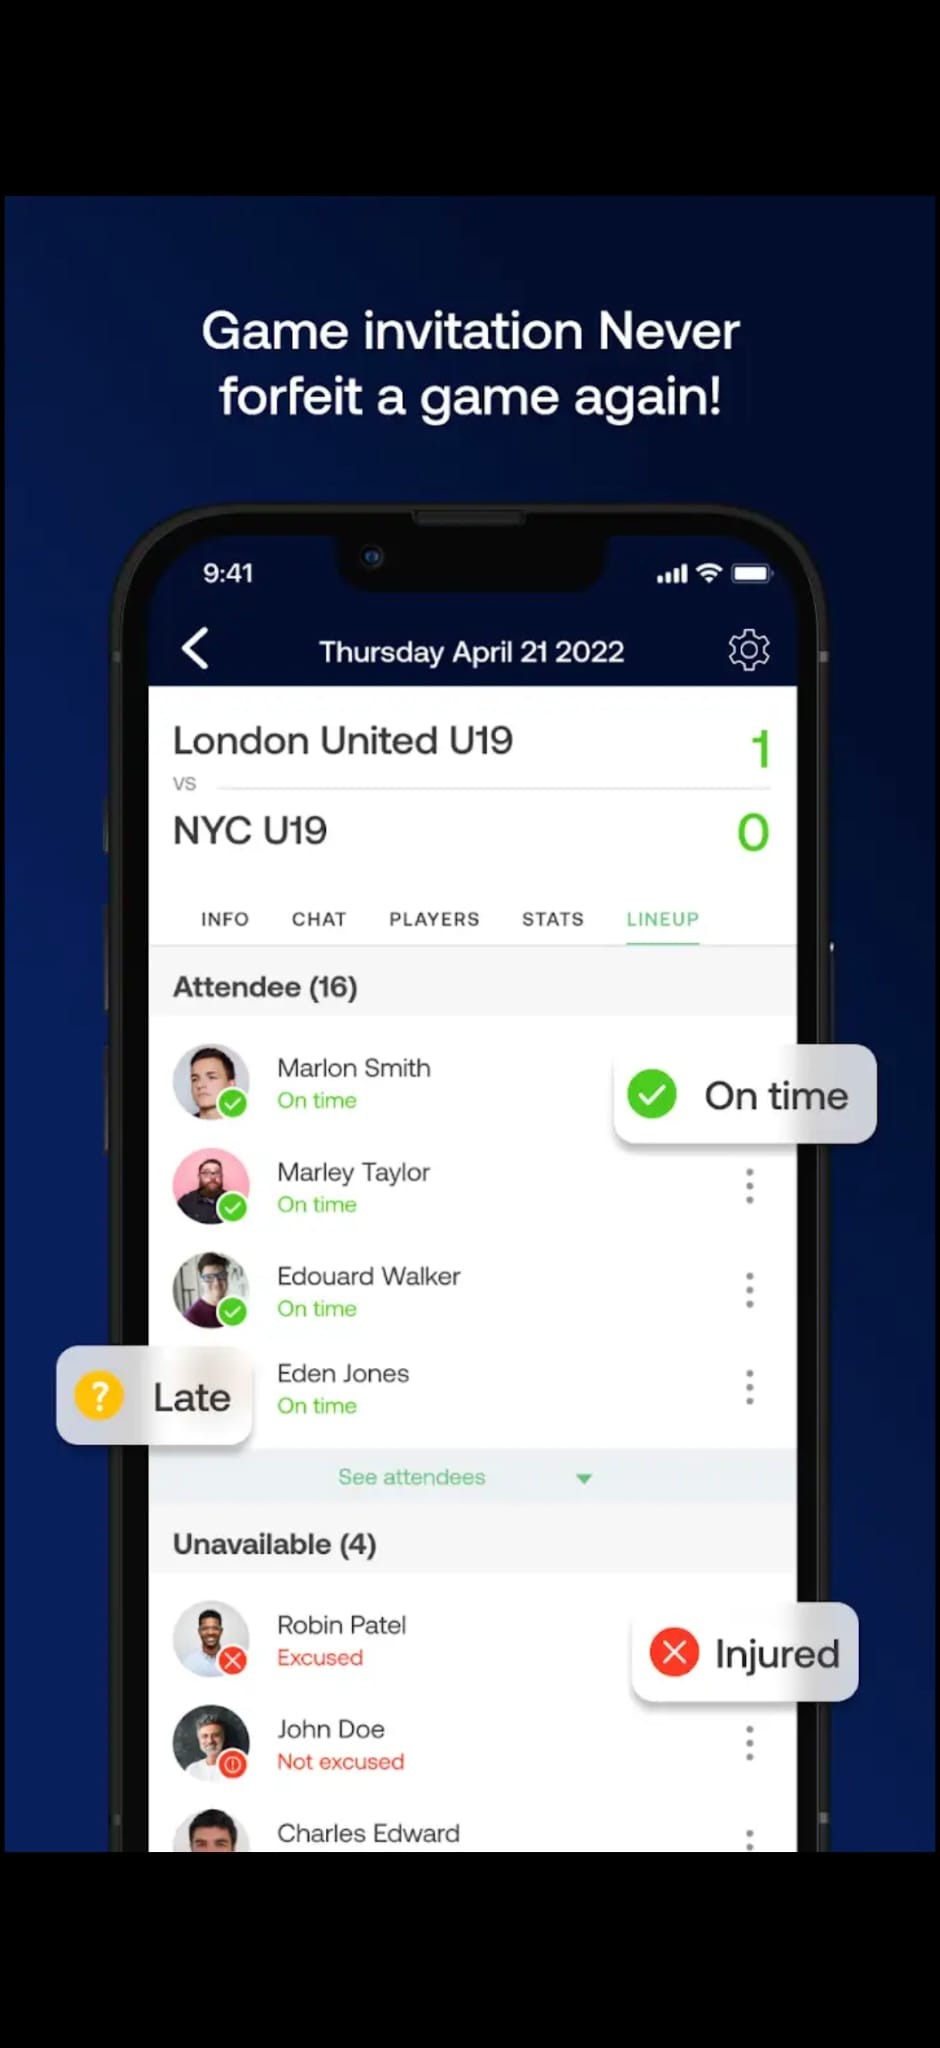
\includegraphics[width=.7\linewidth, height=1.1\linewidth]{imagenes/sportEasy.jpeg}
                \caption{SportEasy \protect\cite{SportEasy}}
                \label{fig:sporteasy_interface}            
            \end{subfigure}\hfill
            \begin{subfigure}{.48\textwidth}
                \centering
                \includegraphics[width=.7\linewidth, height=1.1\linewidth]{imagenes/Playoff.jpeg}
                \caption{Playoff \protect\cite{Playoff}}
                \label{fig:playoff_interface}            
            \end{subfigure}
            
            \vspace{0.5cm} % Espacio vertical entre la primera y segunda fila
            
            % Segunda fila: 2 figuras
            \begin{subfigure}{.48\textwidth}
                \centering
                \includegraphics[width=.7\linewidth, height=1.1\linewidth]{imagenes/TeamSnap.jpeg}
                \caption{TeamSnap \protect\cite{TeamSnap}}
                \label{fig:teamsnap_interface}            
            \end{subfigure}\hfill
            \begin{subfigure}{.48\textwidth}
                \centering
                \includegraphics[width=.7\linewidth, height=1.1\linewidth]{imagenes/Sprongo.jpeg}
                \caption{Sprongo \protect\cite{Sprongo}}
                \label{fig:sprongo_interface}            
            \end{subfigure}
            
            \vspace{0.5cm} % Espacio vertical entre la segunda y tercera fila
            
            % Tercera fila: 1 figura centrada
            \begin{subfigure}{\textwidth}
                \centering
                \includegraphics[width=.33\linewidth, height=0.52\linewidth]{imagenes/Onesporter.jpeg}
                \caption{Onesporter \protect\cite{Onesporter}}
                \label{fig:onesporter_interface}            
            \end{subfigure}
            
            \caption{Interfaces de las soluciones de software analizadas en el estudio competitivo.}
            \label{fig:analisis_competitivo_interfaces}
        \end{figure}

    \section{Objetivos}
    Dado el contexto analizado y las oportunidades de mejora detectadas, estos son los objetivos específicos del proyecto:

    \begin{itemize}
        \item \textbf{Diseñar e implementar la base de datos:} Modelar una estructura relacional en MySQL para almacenar de forma segura y organizada la información de los deportistas, entrenadores, eventos y el histórico de asistencia por temporadas.
        
        \item \textbf{Desarrollo del servicio backend:} Construir una API REST en Node.js con Express estructurada en controladores y rutas independientes para gestionar de manera eficiente todas las peticiones del sistema.
        
        \item \textbf{Garantizar la seguridad mediante roles:} Implementar un sistema de autenticación basado en JSON Web Tokens (JWT) que restrinja el acceso a las rutas del backend según el perfil del usuario (Administrador, Entrenador o Padre).
        
        \item \textbf{Crear la interfaz de usuario móvil:} Desarrollar una aplicación multiplataforma utilizando React Native y Context API que sea ligera, intuitiva y fácil de usar en las condiciones extremas a pie de pista.
        
        \item \textbf{Integrar analítica estadística visual:} Incorporar la librería \textit{react-native-chart-kit} para transformar los registros numéricos de asistencia y entrenamientos en gráficos estadísticos claros que muestren la progresión de los atletas.
        
        \item \textbf{Centralizar la gestión multimedia técnica:} Diseñar un repositorio indexado dentro de la aplicación para que los entrenadores puedan subir fotos y vídeos de los descensos, vinculándolos directamente al perfil de cada deportista para su corrección técnica.
    \end{itemize}

    Con todo ello, la gestión diaria del club de esquí y el seguimiento de los deportistas de base será no solo más eficiente y automatizado, sino también transparente y accesible para los entrenadores y las familias.